\documentclass[11pt]{article}
\usepackage{fancyhdr}
\usepackage{color}
\usepackage{multicol}
\usepackage{fancyvrb}
\usepackage{enumitem}
\usepackage{graphicx}
\usepackage{sectsty}
\usepackage{amsmath}
\usepackage{amssymb}
\usepackage{hyperref}
\usepackage{array}
\newcommand{\sectionbreak}{\clearpage}

\usepackage{tikz}
\usepackage{tkz-euclide}
\usetkzobj{all}

\allsectionsfont{\centering}

\usepackage{draftwatermark}
	\SetWatermarkText{\copyright wolf-math.com}
	\SetWatermarkScale{4}
	\SetWatermarkLightness{1}

\usepackage[margin=1in, headsep=0pt]{geometry}
\setlength{\parindent}{0cm}
\pagestyle{empty}


\begin{document}

Mr. Wolf\\ wolf-math.com

\section*{Introduction to Quadratics}



\subsection*{Goals}

\textbf{SWBAT} multiply monomials into quadratics by using the FOIL method\\

\textbf{SWBAT} multiply the square of a binomial and the difference of squares without using the FOIL method by understanding the pattern of these multiplication problems.\\

\textbf{SWBAT} factor quadratics into the product of two binomials.\\

\textbf{SWBAT} solve a quadratic equation by factoring.\\



\subsection*{Standards}

\textbf{Seeing Structure in Expressions \hfill A-SSE}\\

Write expressions in equivalent forms to solve problems\\

\textbf{3.} Choose and produce an equivalent form of an expression to reveal and explain properties of the quantity represented by the expression.\\
\textbf{a.} Factor a quadratic expression to reveal the zeros of the function it defines\\

\textbf{Reasoning with Equations and Inequalities \hfill A-REI}\\

Understand solving equations as a process of reasoning and explain the reasoning\\

\textbf{4.} Solve quadratic equations in one variable.\\
\textbf{a.} Use the method of completing the square to transform any
quadratic equation in x into an equation of the form (x – p)2 = q
that has the same solutions. Derive the quadratic formula from
this form.\\

\textbf{b.} Solve quadratic equations by inspection (e.g., for x2 = 49), taking
square roots, completing the square, the quadratic formula and
factoring, as appropriate to the initial form of the equation.
Recognize when the quadratic formula gives complex solutions
and write them as a ± bi for real numbers a and b.\\




\subsection*{Connections}

\textbf{Before:} We were learning about linear functions. When two linear functions multiply one another we get a Quadratic function. We are now learning to multiply binomials into quadratics, and factor quadratics into binomials.\\



\textbf{After:} The class will explore completing the square, the quadratic formula, quadratic graphs, and complex numbers (time dependent).\\




\section*{Introduction to Quadratics}

\textbf{Quadratic Function:} a polynomial of degree 2. A quadratic is the result of the product of two linear functions (monomials).\\

\textbf{Multiplying Monomials:}  Use the FOIL technique. \textbf{F}irst \textbf{O}utside \textbf{I}nside \textbf{L}ast\\

\begin{center}
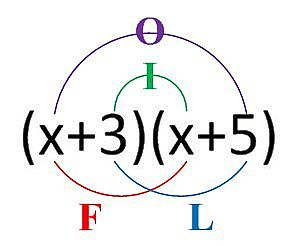
\includegraphics[scale=.5]{foil.jpg}\\
\end{center}

\textbf{Example:} $(x+3)(x+5)$ \\


\textbf{F}irst: $x \cdot x =x^2$\\
\textbf{O}utside: $x \cdot 5 = 5x$\\
\textbf{I}nside: $3 \cdot x = 3x$\\
\textbf{L}ast: $3 \cdot 5 = 15$\\



$= x^{2}+5x+3x+15 = x^{2}+8x+15$\\

\vspace{1in}

\textbf{Your Try:} $(x+2)(x+9)$

\vspace{1in}

\textbf{You Try:} $(x-12)(x+7)$ (\textbf{hint:} the 12 should be treated as a $-12$)\\

\pagebreak

\hrulefill

\textbf{Coefficients on $x$:} The process is the same, but there's a little more to wrangle.\\

\textbf{Example:} $(3x+10)(2x+1)$\\

\vspace{1in}

\textbf{You Try:} $(2x+18)(x+3)$\\

\vspace{1in}

\subsection*{Independent Practice}

\begin{enumerate}
\setlength\itemsep{1cm}
	\begin{multicols}{2}
		\item $(x+1)(x+1)$\\
		
			
		
		\item $(2x+4)(x-7)$\\
		

		
		\item $(2x-1)(x-4)$\\
		
		
		\item $(x-9)(x-4)$\\
		
		
		\item $(3x-4)(x+1)$\\
		
		
		\item $(8x-5)(3x+2)$\\
		
		
		\item $(5x+3)(2x-3)$\\
		
		
		\item $(3x+10)(2x+2)$\\
		
		
	\end{multicols}
\end{enumerate}

\pagebreak

\section*{Multiplying Special Cases}
\subsection*{Square of a Binomial}

The Square of a binomial looks like

$$(a+b)^2$$

$$(a+b)^2 \neq (a^2+b^2)$$

Think Pythagorean Theorem for the reason.\\

To obtain the correct value we need to FOIL. The meaning of $(x+5)^2$ is $(x+5)(x+5)$\\

$$(x+5)^2= x^2+10x+25$$\\

\textbf{General Rule:} $(a+b)^2= \mathbf{a^2+2ab+b^2}$\\

\textbf{Example:} $(2q-9)^2=4q^2-36q+81$\\

Use this pattern to simply convert the square of a binomial without actually FOILing.\\

\textbf{You Try:} Expand the problems without using FOIL.\\
\begin{enumerate}
	\begin{multicols}{2}
	
		\item $(f+2)^2=$\\
		
			\vspace{1cm}
		
		\item $ (h-3)^2=$\\
		
			\vspace{1cm}
		
		\item $ (3p+7)^2=$\\
		
			\vspace{1cm}
		
		\item $ (4g-5)^2=$\\
		
			\vspace{1cm}
		
		\item $(x+y)^2=$\\
		
			\vspace{1cm}
		
		\item $(h-k)^2=$\\
		
			\vspace{1cm}
		
		\item $(2m+n)^2=$\\
		
			\vspace{1cm}
		
		\item $(3u-v)^2=$\\
		
			\vspace{1cm}
		
		\item $(3a+6b)^2=$\\
		
			\vspace{1cm}
		
		\item $(5r-10s)^2=$\\

	\end{multicols}
\end{enumerate}

\pagebreak

\subsection*{Difference of Squares}

$$a^2-b^2$$

This is called the \textbf{difference of squares} because the $a$ is squared, the $b$ is also squared, and they are subtracted (difference). \\

This happens when you multiply 2 special binomials. 

$$(a+b)(a-b)= \mathbf{a^2-b^2}$$\\

\textbf{Example:} Foil the following $(x+2)(x-2)$\\

$$(x^2-2x+2x-4)$$

Notice the middle terms $(-2x+2x)$ cancel out. The first term $x^2$ and last term $4$ are both perfect squares.  They have subtraction in between them, hence the "difference" in \textbf{difference of squares}.

Thus, our answer is 

$$\mathbf{x^2-4}$$

\textbf{You Try:} Rewrite the expression as a difference of squares.\\

\begin{enumerate}
	\begin{multicols}{2}
	
		\item $(h-3)(h+3)=$\\
		
			\vspace{1cm}
		
		\item $(j+10)(j-10)$\\
		
			\vspace{1cm}
		
		\item $(2k-5)(2k+5)$\\
		
			\vspace{1cm}
		
		\item $(9g-9)(9g+9)$\\
		
			\vspace{1cm}
		
	\end{multicols}
\end{enumerate}

You can go in the opposite direction too. If you have a difference of squares you can write a product of binomials.\\

$$25x^2-16 = (5x-4)(5x+4)$$

\textbf{You Try:} Convert from a difference of squares to the product of binomials.\\

\begin{enumerate}
	\begin{multicols}{2}

		\item $n^2-100$\\
		
		\item $p^2-64$\\
		
		\item $4r^2-16$\\
		
		\item $9m^2-81w^2$\\

	\end{multicols}
\end{enumerate}

\pagebreak

\section*{Factoring Trinomials}

We know how to multiply 2 binomials into a trinomial by using the FOIL method. Now we're going to \textit{factor} the trinomial back into two binomials.\\

\textbf{Example 1:}

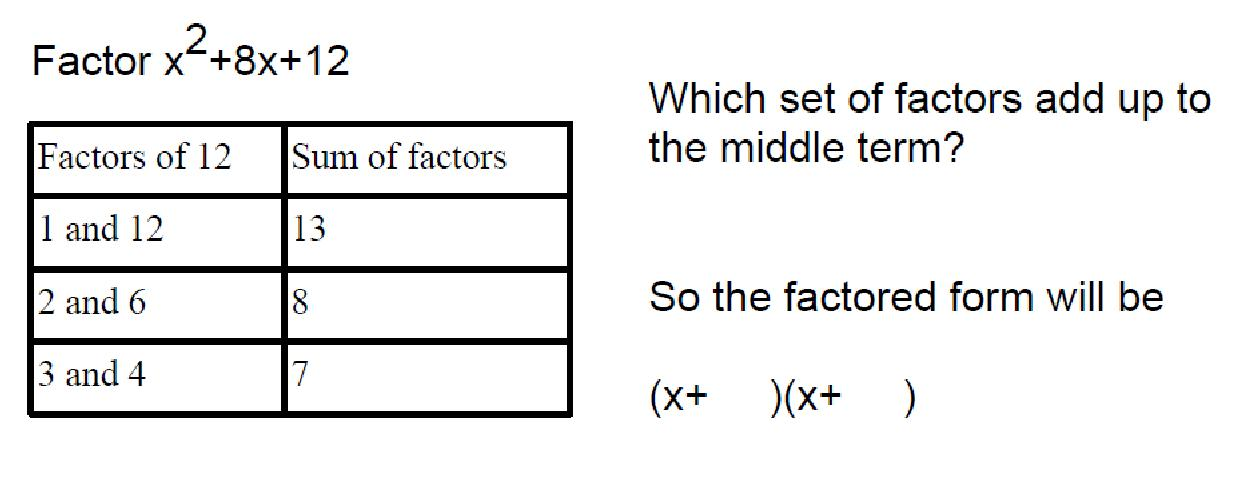
\includegraphics[scale=.25]{factor1.jpg}

\hrulefill

\textbf{Example 2:}\\

Factor $x^2+9x+20$\\

\vspace{1in}

$$(x+\hspace{.5cm})(x+\hspace{.5cm})$$

\hrulefill

\textbf{You Try:}

Factor $x^2+11x+18$\\


\pagebreak


\subsection*{Negatives in Trinomials}


When there is a negative in the \textit{second spot} or in \textit{both spots} that means that there is \textbf{1 negative}.\\

$x^2+5x-50$ -- Bigger factor is \textbf{negative}\\

$50=2\cdot25$\\ \hspace{1cm}$5\cdot10$\\

Which two of these subtracted from each other $=+5$?\\

$(x+10)(x-5)$\\

\textbf{You Try:} Factor $x^2+5x-14$

\vspace{.75in}


\hrulefill

$x^2-4x-12$ -- Smaller factor is \textbf{negative}\\

$12=2\cdot 6$\\ \hspace{1cm}$3\cdot4$\\

Which two of these subtracted from each other $=-4$?\\

$(x+2)(x-4)$\\

\textbf{You Try:} Factor $x^2-x-20$\\

\vspace{.75in}

\hrulefill

When the first sign is \textbf{ negative} then that means \textbf{BOTH FACTORS} are negative.\\

$x^2-6x+8$ \\

$8=2\cdot 4$\\

$(x-2)(x-4)$\\

\textbf{You Try:} Factor $x^2-12x+36$\\

\pagebreak

\section*{Quiz Review -- Trinomials}

Mr. Wolf \hfill NAME:\underline{\hspace{3in}}\\ 
Algebra 2 \\ 
CMSD-JFK \hfill DATE:\underline{\hspace{2in}}\\
2014-2015\\



\textbf{Multiply the binomials into a trinomial by using the FOIL technique}\\

\begin{enumerate}
	\begin{multicols}{2}
	
		\item $(x+5)(x+3)$\\
		
		\item $(h-4)(h+6)$\\
		
		\item $(k-2)(k-8)$\\
		
		\item $(3p+4)(p+2)$\\
		
		\item $(4y+1)(2y+3)$\\
		
		\item $(2r+s)(3r-s)$\\
		
	\end{multicols}
\end{enumerate}

\hrulefill

\textbf{Multiply the binomials into trinomials without using the FOIL technique. Notice the \textit{square of a binomial} and the \textit{difference of squares.}}\\

\begin{enumerate}[resume]
	\begin{multicols}{2}
			\item $(x+4)^2$\\
			
			\item $(g+5)^2$\\
			
			\item $(k-7)^2$\\
			
			\item $(2p+3)^2$\\
			
			\item $(3t-3)^2$\\
			
			\item $(5y-4f)^2$\\
			
			\item $(q+1)(q-1)$\\
			
			\item $(10p-10)(10p+10)$\\
			
			\item $(d-4)(d+4)$\\
			
			\item $(r+4)(r-4)$\\
			
			\item $(2v-9)(2v+9)$\\
			
			\item $(7i-j)(7i+j)$\\
			
			\item $(m+n)(m-n)$\\
	\end{multicols}
\end{enumerate}

\pagebreak

\textbf{Factor the trinomials into the product of two binomials}\\


\begin{enumerate}[resume]
	\begin{multicols}{2}
	
		\item $x^2+21x+20$\\
		
		
		\item $x^2+9x+20$\\
		
		
		\item $x^2+13x+30$\\
		
		
		\item $x^2+11x+30$\\
		
		
		\item $x^2-8x+12$\\
		
		
		\item $x^2-7x+12$\\
			
	
	\end{multicols}
\end{enumerate}

\pagebreak

\section*{Quiz Trinomials -- OPEN NOTE}

Mr. Wolf \hfill NAME:\underline{\hspace{3in}}\\ 
Algebra 2 \\ 
CMSD-JFK \hfill DATE:\underline{\hspace{2in}}\\
2014-2015\\



\textbf{Multiply the binomials into a trinomial by using the FOIL technique}\\

\begin{enumerate}
	\begin{multicols}{2}
	
		\item $(x+4)(x+2)$\\
		
		\item $(h-3)(h+5)$\\
		
		\item $(k-3)(k-9)$\\
		
		\item $(2p+5)(p+3)$\\
		
		\item $(5y+2)(3y+4)$\\
		
		\item $(3r+s)(4r-s)$\\
		
	\end{multicols}
\end{enumerate}

\hrulefill

\textbf{Multiply the binomials into trinomials without using the FOIL technique. Notice the \textit{square of a binomial} and the \textit{difference of squares.}}\\

\begin{enumerate}[resume]
	\begin{multicols}{2}
			\item $(x+54)^2$\\
			
			\item $(g+6)^2$\\
			
			\item $(k-8)^2$\\
			
			\item $(2p+4)^2$\\
			
			\item $(3t-4)^2$\\
			
			\item $(4y-5f)^2$\\
			
			\item $(q+2)(q-2)$\\
			
			\item $(10p-11)(10p+11)$\\
			
			\item $(d-5)(d+5)$\\
			
			\item $(r+6)(r-6)$\\
			
			\item $(2v-8)(2v+8)$\\
			
			\item $(6i-j)(6i+j)$\\
			
			\item $(m+2n)(m-2n)$\\
	\end{multicols}
\end{enumerate}

\pagebreak

\textbf{Factor the trinomials into the product of two binomials}\\


\begin{enumerate}[resume]
	\begin{multicols}{2}
	
		\item $x^2+17x+16$\\
		
		
		\item $x^2+10x+16$\\
		
		
		\item $x^2+10x+21$\\
		
		
		\item $x^2+22x+21$\\
		
		
		\item $x^2-11x+24$\\
		
		
		\item $x^2-10x+24$\\
			
	
	\end{multicols}
\end{enumerate}

\pagebreak

\section*{Factoring Trinomials $a>1$}

$$ax^2+bx+c$$

We know how to factor a trinomial when $a=1$. That means that there is no coefficient in front of the $a^2$ term. However, it can be factored but it takes a little bit more effort.\\

\begin{large}
\textbf{When there is a common factor:} If there is a common factor between all of the terms of the trinomial, then it can be factored out. \\
\end{large}

\textbf{Example 1:} Factor $2x^2+10x+8$ \\

The coefficients are 2,10, and 8. Since 2 can go into all of those numbers it can be pulled out.\\

$2(x^2+5x+4)$\\

Now we notice that $(x^2+5x+4)$ can be further factored. So our end result is.\\

$2(x+4)(x+1)$\\


\textbf{Example 2:} Factor $3x^2+15x+18$\\

\vspace{1in}

\textbf{You Try:} Factor $2x^2+16x+30$\\

\vspace{1in}

Factor $5x^2-2x-12$\\

\pagebreak

\section*{Diamond Method of Factoring}

Use the diamond method to factor $2x^2+7x+3$\\

\begin{center}

\includegraphics[scale=.5]{diamond.jpg}
\end{center}

\vspace{1cm}

\textbf{Answer:}

\hrulefill

\textbf{Factor:} $3x^2+8x+4$\\

\begin{center}

\includegraphics[scale=.5]{diamond.jpg}
\end{center}

\pagebreak

\section*{Solving Quadratics by Factoring}

We know how to solve equations like $5x+7=52$\\

You may even know how to solve an equation like $x^2=9$\\

But how do you solve an equation like $x^2+21x=-20$? There are no like-terms to combine, you can't isolate an $x$ to solve it! The answer is to \textit{FACTOR} (everyone's favorite past-time). \\

Follow these 5 steps to solve \\

	\begin{enumerate}
		\item Make one side of the equals sign $0$\\
		
		\item Factor\\
		
		\item Solve each of the factors alone\\
		
		\item You have 1 \textit{or} 2 answers\\
		
		\item Check your answer\\
	\end{enumerate}

\textbf{Example 1:} $x^2+21x=-20$

	\begin{enumerate}
		\item $ x^2+21x+20=0$\\
		
		\item $ (x+20)(x+1)=0$\\
		
		\item 	\begin{enumerate}
			\item $x+20=0$\\
			
			\item $x+1=0$ \\
			
		\end{enumerate}
		
		\item  \begin{enumerate}
			\item  $x=-20$\\
			
			\item $x=-1$\\
		\end{enumerate}
		
		
		\item \begin{enumerate}
			\item $(-20)^2+21(-20)+20=0$\\
			
			\item $(-1)^2+21(-1)+20=0$\\
		\end{enumerate}
	\end{enumerate}

\pagebreak

\textbf{Example 2:} $x^2+9x=-20$\\


\vspace{2in}

\textbf{Example 3:} $-x^2=13x+30$\\

\vspace{2in}

\textbf{You Try:} $x^2+11x+30=0$\\

\vspace{2in}

$x^2-8x=-12$

\pagebreak

Solving equations practice\\

$(x+1)(x+1)=0$\\
		
		
		
$(2x+4)(x-7)=0$\\


$x^2-8x=-12$\\
		
		
$x^2=+7x-12$\\


$2x^2+16x+30=0$\\


 $5x^2-2x=12$\\
 
 $2x^2+7x=-3$\\
 
 $3x^2+13x+10=5x+6$

\pagebreak

\section*{Quiz Review -- Factoring \& Solving Quadratics}


Mr. Wolf \hfill NAME:\underline{\hspace{3in}}\\ 
%Algebra 2 \\ 
%CMSD-JFK \hfill DATE:\underline{\hspace{2in}}\\
%2014-2015\\



\textbf{Factor the Trinomials $a=1$}\\

\begin{enumerate}
\begin{multicols}{2}

\item $x^2+6x+5$\\

	\vspace{1cm}

\item $x^2+8x+12$\\

	\vspace{1cm}

\item $x^2-99x-100$\\

	\vspace{1cm}

\item $x^2-28x+75$\\

	\vspace{1cm}

\end{multicols}
\end{enumerate}

\hrulefill

\textbf{Factor the Trinomials $a>1$} -- Factor out a common factor\\

\begin{enumerate}[resume]
\begin{multicols}{2}

\item $3x^2+9x+6$\\

	\vspace{1cm}

\item $2x^2+14x+20$\\

	\vspace{1cm}

\item $5x^2-75x-500$\\

	\vspace{1cm}

\item $3x^2-60x+225$\\

	\vspace{1cm}

\end{multicols}
\end{enumerate}


\hrulefill

\textbf{Factor the Trinomials $a>1$} -- Diamond Method or Factor by grouping\\

\begin{enumerate}[resume]
\begin{multicols}{2}

\item $2x^2+7x+5$\\

	\vspace{1cm}

\item $6x^2+11x+3$\\

	\vspace{1cm}

\item $2x^2+13x-7$\\

	\vspace{1cm}

\item $5x^2+18x+9$\\

	\vspace{1cm}

\end{multicols}
\end{enumerate}



\pagebreak

\textbf{Solve the Quadratic Equations} 

\begin{enumerate}[resume]

\item $(x-2)(x+5)=0$\\

	\vspace{1cm}
	
\item $(3x-9)(x+5)=0$\\

	\vspace{1cm}

\item $x^2+6x+5=0$\\

	\vspace{1cm}

\item $x^2-99x=100$\\

	\vspace{1cm}

\item $x^2+6x+105=100$\\

	\vspace{1cm}

\item $2x^2+7x+5=0$\\

	\vspace{1cm}

\item $6x^2+11x+9=6$\\

	\vspace{1cm}

\item $2x^2+13x=7$\\
\end{enumerate}

\pagebreak

\section*{Quiz  -- Factoring \& Solving Quadratics}

Mr. Wolf \hfill NAME:\underline{\hspace{3in}}\\ 
%Algebra 2 \\ 
%CMSD-JFK \hfill DATE:\underline{\hspace{2in}}\\
%2014-2015\\

\begin{center}
		\textbf{OPEN NOTE}\\
\end{center}

\vspace{1cm}

\textbf{Factor the Trinomials $a=1$}\\

\begin{enumerate}
\begin{multicols}{2}

\item $x^2+3x+2$\\

	\vspace{1cm}

\item $x^2+7x+10$\\

	\vspace{1cm}

\item $x^2-15x-100$\\

	\vspace{1cm}

\item $x^2-20x+75$\\

	\vspace{1cm}

\end{multicols}
\end{enumerate}

\hrulefill

\textbf{Factor the Trinomials $a>1$} -- Factor out a common factor\\

\begin{enumerate}[resume]
\begin{multicols}{2}

\item $2x^2+6x+4$\\

	\vspace{1cm}

\item $3x^2+21x+30$\\

	\vspace{1cm}

\item $4x^2-60x-400$\\

	\vspace{1cm}

\item $2x^2-40x+150$\\

	\vspace{1cm}

\end{multicols}
\end{enumerate}


\hrulefill

\textbf{Factor the Trinomials $a>1$} -- Diamond Method or Factor by grouping\\

\begin{enumerate}[resume]
\begin{multicols}{2}

\item $2x^2+5x+3$\\

	\vspace{1cm}

\item $3x^2+5x-2$\\

	\vspace{1cm}

\item $3x^2+13x-10$\\

	\vspace{1cm}

\item $2x^2-11x+14$\\

	\vspace{1cm}

\end{multicols}
\end{enumerate}



\pagebreak

\textbf{Solve the Quadratic Equations} -- BOOM!

\begin{enumerate}[resume]

\item $(x-1)(x+1)=0$\\

	\vspace{1cm}
	
\item $(2x-8)(x+10)=0$\\

	\vspace{1cm}

\item $x^2+3x+2=0$\\

	\vspace{1cm}

\item $x^2+7x=-10$\\

	\vspace{1cm}

\item $x^2=15x+100$\\

	\vspace{1cm}

\item $x^2-20x+90=15$\\

	\vspace{1cm}

\item $2x^2+5x+3=0$\\

	\vspace{1cm}

\item $3x^2+5x=2$\\
\end{enumerate}

\vspace{1in}

Now you're done :-)

\end{document}